\documentclass[10pt,letterpaper]{bp-template-concise}

\begin{document}

% ============================================================
% TITLE
% ============================================================
\leftalignedtitle{Mandatory Disclosure and Housing Market Dynamics}

\leftalignedauthor{
    Bastien Patras, \href{mailto:bastien.patras@sciencespo.fr}{bastien.patras@sciencespo.fr}$^\dagger$\\
    {\small $^\dagger$PhD Student, Sciences Po Department of Economics, Paris, France}\\
}
\vspace{1em}

\abs{
\textbf{Abstract}\\[0.5em]
Standard unraveling theory predicts that mandatory disclosure separates high-quality from low-quality products. We document a puzzle in the French housing market: following the 2021 enforcement of mandatory Energy Performance Certificate (EPC) disclosure, properties listed without EPC scores trade at a 6 percentage point premium over energy-efficient properties that disclose---the opposite of what classical theory and the existing EPC literature predict. We develop a model in which unraveling fails because non-disclosure pools two economically distinct populations: informed sellers strategically concealing unfavorable information, and uninformed sellers who genuinely do not know their property's energy performance. When buyers cannot distinguish between these groups, silence becomes ambiguous rather than damning, and low-quality sellers benefit from pooling with the genuinely uninformed. We show that the market's ability to price quality information depends on the composition of both sides: the share of informed sellers ($\pi$) and the share of quality-sensitive buyers ($\rho$). Full unraveling requires both to be high; for intermediate values, non-disclosure premia persist in equilibrium. We identify the model using a unique combination of residential listing records, transaction data, and the ADEME registry of certified energy audits---a third-party database that lets us directly observe each seller's information status at listing time, the latent variable that buyers cannot see. Our framework generates a closed-form optimal subsidy formula for energy renovations that varies with local market composition, and reveals a novel policy equivalence: tightening disclosure enforcement and increasing renovation subsidies are perfect substitutes at the margin, making uniform national policies generically inefficient.
}

\vspace{1em}
\keywords{Energy Performance Certificates, Mandatory Disclosure, Housing Markets, Unraveling, Information Asymmetry} \\
\vspace{0.2em}
\jel{Q48, R31, Q52, D83, R38, H23}

% ============================================================
\section{Introduction}
% ============================================================

Standard unraveling theory offers a stark prediction: in markets with verifiable quality information, sellers with good products disclose, silence signals bad news, and disclosure unravels until it is effectively universal \citep{grossman_informational_1981,milgrom_good_1981}. The French housing market presents a sharp challenge to this view. Since 2021, France has required sellers to disclose Energy Performance Certificate (EPC) scores in all property listings. Yet four years after implementation, a substantial fraction of listings still omit this information, and these non-disclosing properties trade at a \textit{premium} over properties that disclose balanced ratings (see chapter 1, and Figure \ref{fig:ATT}). The market does not punish opacity---it rewards it.

The puzzle is sharpened by the broader empirical record on energy labels in housing markets. A large body of work establishes that energy-efficient properties command meaningful price premia wherever EPCs have been studied: \citet{brounen_kok_2011} document a 2--5\% premium for A/B-rated homes in the Netherlands following that country's 2008 mandate; \citet{hyland_lyons_2013} find premia of up to 9\% in Ireland; \citet{fuerst_energy_2016} confirm similar gradients in Wales; \citet{frondel_power_2018} show that Germany's shift from voluntary to mandatory disclosure reduced prices for non-disclosed listings, precisely as classical theory predicts; and \citet{myers_mandatory_2022} demonstrate that mandatory disclosure requirements in the United States increase the capitalization of energy efficiency and stimulate renovation investment. The consensus reading of this literature is that EPC mandates make quality salient, rewarding efficiency and penalizing waste. What none of these papers can explain is why \emph{silence}---the deliberate omission of an EPC score---commands a premium. If anything, it should be the worst signal of all.

The gap lies in a foundational assumption that the classical framework and the EPC literature share: non-disclosure is always a \emph{choice}. A seller who has not yet obtained a certified energy audit cannot disclose, regardless of her property's true performance. \citet{dye_disclosure_1985} first identified this distinction in the context of corporate earnings announcements, showing that when firms may simply lack private information, the market cannot interpret silence as unambiguously bad news. \citet{jung_kwon_1988} formalize the resulting equilibria: partial pooling---in which strategically hiding low-quality sellers shelter behind genuinely uninformed non-disclosers---is generically stable. When buyers observe a missing EPC score, they face irreducible ambiguity: they cannot determine whether the seller is concealing unfavorable information or simply lacks a certified audit. Silence becomes \textit{noise}, not a signal, and its informativeness depends entirely on the composition of the non-disclosing pool.

Yet Dye-type models are set in corporate finance and accounting, where investors are treated as homogeneous in how much they value the disclosed signal. Housing markets are fundamentally different. A buyer purchasing a vacation property in the south of France, occupied a few weeks per year, may rationally ignore EPC scores; a buyer of a primary residence in northern France with cold winters will price energy costs directly. \citet{loewenstein_disclosure_2014} survey evidence that disclosure interventions systematically fail when recipients are inattentive or heterogeneous in their responses; \citet{benshahar_failure_2011} document this pattern across many regulated markets, from mortgage disclosures to nutritional labels; and \citet{fishman_mandatory_2003} show formally that mandatory disclosure can be ineffective---or even welfare-reducing---when buyers differ in their capacity to process the disclosed information. When a large share of buyers is effectively indifferent to the EPC signal, the revenue penalty from concealment is diluted, sustaining hiding even when buyers hold pessimistic beliefs about the non-disclosing pool.

We formalize this intuition in a model with two key departures from the classical framework. First, we allow for \textbf{seller heterogeneity in information}: some sellers know their property's energy performance, while others do not. Second, we allow for \textbf{buyer heterogeneity in preferences}: some buyers care about energy efficiency, while others do not. These two dimensions, parameterized by $\pi$ (the share of informed sellers) and $\rho$ (the share of quality-sensitive buyers), jointly determine whether markets unravel, partially separate, or sustain pooling equilibria with premia to opacity. When both $\pi$ and $\rho$ are high, the classical benchmark is recovered. For intermediate values---our empirically relevant regime---partial separation with a persistent non-disclosure premium is the generic outcome.

A distinctive feature of this paper is the vantage point from which we observe the disclosure game. Testing a theory of strategic concealment requires seeing both sides of the information asymmetry simultaneously: the seller's true information, the seller's strategic choice, and the market's response. Most empirical work in this space sees only one or two of these. Studies of information asymmetry in housing infer agent advantages from equilibrium price deviations \citep{levitt_syverson_2008}; analyses of certification intermediaries characterise incentives without observing individual information endowments \citep{lizzeri_1999}; and work on the energy efficiency gap must proxy for seller awareness through indirect variation in energy prices \citep{myers_asymmetric_2020}. We observe all three dimensions directly. Our dataset combines (i)~\textbf{residential listing records} covering hundreds of thousands of French properties, with listing prices, characteristics, and each seller's disclosure decision; (ii)~\textbf{transaction records} capturing actual sale prices and time-on-market, allowing us to trace the market's response from listing through closing; and (iii)~the \textbf{ADEME registry of certified energy audits}, an official third-party database maintained by France's environment and energy management agency, compiled independently of the listing market. By matching properties across all three sources, we directly observe the latent variable $K_i$---whether a seller possesses a certified audit at listing time---that buyers can never see. This lets us classify every listing into one of four empirically meaningful groups: truthful disclosers, strategic hiders (informed sellers with a certified audit who omit it), genuinely uninformed sellers (no audit exists), and the rare misreporters (audit exists but displayed score diverges). The result is a dataset in which the full information structure of the disclosure game is observed, not inferred---a vantage point that, to our knowledge, is unique in the empirical disclosure literature.

We then extend the model to a policy context. When energy performance is endogenous---sellers can undertake costly renovation---the non-disclosure premium creates a private incentive to conceal rather than upgrade. Concealment and renovation become strategic substitutes: the non-disclosure premium acts as an implicit subsidy to inefficiency. This is a new, information-based mechanism for the energy efficiency gap that \citet{allcott_is_2012} and \citet{gerarden_assessing_2017} identify as one of the central puzzles in energy economics. The distortion further rationalizes the documented free-riding in France's renovation tax credits \citep{nauleau_2014}: uniform national subsidies are misaligned with the cross-market variation in $(\pi,\rho)$ that determines how strongly private incentives already discipline strategic concealment. Our model delivers a closed-form optimal subsidy $S^*(\pi,\rho,X)$ and a novel equivalence result absent from existing policy frameworks \citep{gillingham_palmer_2014}: tightening disclosure enforcement and increasing renovation subsidies are \textit{perfect substitutes at the margin}---each euro of additional hiding cost reduces the required subsidy by exactly one euro.

% ============================================================
\section{Research Questions}
% ============================================================

The empirical puzzle motivates three interconnected questions that this paper addresses in sequence. The first is theoretical---what breaks the classical mechanism? The second is positive---what determines equilibrium outcomes and how can they be identified? The third is normative---how should policy respond?

\vspace{0.5em}

\noindent\textbf{RQ1. Why does mandatory disclosure fail to unravel the market?}

\vspace{0.2em}

\noindent \citet{grossman_informational_1981} and \citet{milgrom_good_1981} establish that rational markets can achieve full disclosure without any mandate: sellers with good products voluntarily reveal, silence unravels until it is fully revealing of low quality, and laws merely accelerate what competition achieves on its own. The broader EPC literature---documenting green premia in the Netherlands \citep{brounen_kok_2011}, Ireland \citep{hyland_lyons_2013}, Wales \citep{fuerst_energy_2016}, Germany \citep{frondel_power_2018}, and the United States \citep{myers_mandatory_2022}---implicitly assumes this mechanism is operative: mandates work because silence is punished. The French evidence breaks this assumption. The first question is therefore: \textit{under what conditions does the classical unraveling logic break down, and what sustains pooling equilibria in which silence is rewarded rather than penalized?}

The paper's answer rests on two conditions that both fail simultaneously. First, sellers must \textit{know} their quality in order to disclose it. Energy audits in France require costly third-party certification; sellers under time pressure (relocation, financial distress, inheritance) may list before completing one. Non-disclosure then reflects genuine informational constraint, not strategic concealment---precisely the mechanism identified by \citet{dye_disclosure_1985} and \citet{jung_kwon_1988} in the accounting literature, and transplanted here to housing markets for the first time. Second, buyers must \textit{value} the disclosed information. When buyers are heterogeneous in energy-cost sensitivity---varying with climate, income, occupancy, and energy prices---a substantial share of the market is effectively indifferent to EPC scores, diluting the revenue penalty from concealment \citep{fishman_mandatory_2003,loewenstein_disclosure_2014}. Either failure is sufficient to prevent unraveling; together, they generate robust pooling equilibria with persistent non-disclosure premia.

\vspace{0.8em}

\noindent\textbf{RQ2. How do market composition and hiding costs determine equilibrium outcomes?}

\vspace{0.2em}

\noindent Given that unraveling can fail, the second question is positive: \textit{what determines the size of the non-disclosure premium, whether it persists in equilibrium, and how it varies across markets?}

The model characterizes equilibrium as a function of three primitives: $\pi$ (the fraction of sellers who are informed at listing time), $\rho$ (the fraction of buyers who are EPC-sensitive), and $c_0$ (the cost of non-disclosure, capturing regulatory enforcement stringency). Higher $\pi$ erodes the premium---buyers correctly infer that uninformed sellers are rare and that most non-disclosers are strategic hiders, making silence more damning. Higher $\rho$ amplifies it---the revenue difference between a disclosed high-quality listing and a hidden low-quality listing grows, making concealment more attractive even when buyer beliefs are pessimistic. Higher $c_0$ directly suppresses it by raising the cost of hiding. The model delivers a complete comparative-static characterization and a closed-form expression for the non-disclosure premium as a function of $(\pi, \rho, c_0)$.

We identify these parameters empirically using the unique structure of our dataset. Matching residential listings against the ADEME registry of certified energy audits allows us to directly observe $K_i$---each seller's information status at listing time---which buyers can never see and which existing studies must infer from equilibrium outcomes \citep{levitt_syverson_2008,myers_asymmetric_2020}. Combined with transaction records capturing actual sale prices, we separately measure the behavior of informed and uninformed sellers, and estimate $\pi$, $\rho$, and $c_0$ at the market level using a difference-in-differences design around the July 2021 reform.

\vspace{0.8em}

\noindent\textbf{RQ3. What is the optimal renovation subsidy, and why are uniform national policies inefficient?}

\vspace{0.2em}

\noindent The third question is normative: \textit{when sellers can invest in energy renovations, how should subsidies be designed to correct the distortion created by the non-disclosure premium?}

The non-disclosure premium makes concealment and renovation strategic substitutes: a seller with a low-quality property can either pay to hide or pay to upgrade. The premium acts as an implicit subsidy to inefficiency, generating a new information-based mechanism for the energy efficiency gap \citep{allcott_is_2012,gerarden_assessing_2017}. The paper extends the model to endogenous quality and derives a closed-form optimal subsidy $S^*(\pi,\rho,X)$ equal to the gap between actual renovation costs and the market-implied renovation threshold. The formula has two striking properties. First, the required subsidy is decreasing in both $\pi$ and $\rho$: markets where informational conditions already discipline strategic hiding need less fiscal support. Second, and more surprisingly, disclosure enforcement and renovation subsidies are \textit{perfect substitutes at the margin}---each euro of increased hiding cost reduces the required subsidy by exactly one euro. This equivalence, absent from existing policy frameworks \citep{gillingham_palmer_2014}, directly rationalizes the documented free-riding in France's uniform renovation tax credits \citep{nauleau_2014}: a national subsidy that ignores cross-market heterogeneity in $(\pi,\rho)$ over-subsidizes markets where private incentives are already strong and under-subsidizes those where disclosure frictions are most severe.

% ============================================================
\section{Why Unraveling Fails}
% ============================================================

The classical unraveling argument rests on two implicit assumptions: sellers know their quality, and buyers value disclosed information. When either fails, the logic breaks down.

\textbf{Sellers may not know their quality.} Energy performance requires costly third-party certification. Sellers under time pressure (relocation, financial distress, inheritance) may list before completing an audit. Non-disclosure then may reflect a genuine informational constraint rather than strategic concealment. The fraction of sellers who are informed at the time of listing, $\pi$, is shaped by market infrastructure and local audit capacity (not solely by seller preferences.

\textbf{Buyers may not care.} A buyer purchasing a vacation home in the south of France, occupied only a few weeks per year, may rationally ignore EPC scores. A buyer of a primary residence in northern France with cold winters will incorporate energy costs directly into willingness to pay. The fraction of quality-sensitive buyers, $\rho$, varies with climate, income, occupancy, and energy prices.

\textbf{Both conditions are needed for unraveling.} When $\rho=0$, disclosure decisions are economically irrelevant (buyers do not respond). When $\pi=0$, non-disclosure is universal and carries no adverse inference (buyers understand it reflects constraint, not concealment. Only when both parameters are interior does partial unraveling occur: some informed sellers disclose, some hide, and uninformed sellers provide cover for the hiders, sustaining a pooling premium.

% ============================================================
\section{Model}
% ============================================================

\subsection{Environment and Timing}

A seller owns a property with observable attributes $X$ and an unobservable energy performance level $\theta \in \{0,1\}$, where $\theta=1$ denotes high efficiency. With probability $\pi\in(0,1)$, the seller is \emph{informed} and knows $\theta$; with probability $1-\pi$, she is \emph{uninformed}. The seller simultaneously chooses a disclosure decision $d\in\{0,1\}$ and a listing price $p^{\text{list}}$. Uninformed sellers are constrained to $d=0$.

A buyer then arrives, observes $(d,p^{\text{list}},X)$, and decides whether to purchase at $p^{\text{list}}$. With probability $\rho\in(0,1)$, the buyer is \emph{EPC-sensitive} and values energy efficiency; with probability $1-\rho$, the buyer is \emph{EPC-insensitive}. Sellers cannot observe buyer type ex ante and optimize against expected demand.

We provide a visual representation of the model dynamics and Timing in Figure \ref{fig:vis_model}.

\subsection{Payoffs and Hiding Costs}

The seller's optimization problem is:
\begin{equation}
    \max_{\{d,\,p^{\text{list}}\}} \;\Pi = \underbrace{\mathbb{E}\!\left[p^{\text{trans}}\mid d,p^{\text{list}},X\right]}_{\phi(p^{\text{list}})} \cdot \underbrace{\Pr(T{=}1\mid d,p^{\text{list}},X)}_{\Gamma(p^{\text{list}})} - C(\theta,d)
    \label{eq:payoff}
\end{equation}

\begin{itemize}
    \item $\phi(p^{\text{list}}) = \gamma_0+\gamma_1 \cdot p^{\text{list}}+\sum_n\gamma_n X_n$ is the expected transaction price conditional on a sale occurring
    \item $C(\theta,d)=\mathbf{1}[d=0]\cdot(c_0+\theta c_1)$ is the hiding cost which is only paid when the seller withholds information
\end{itemize}

 The term $c_0\geq 0$ applies to all non-disclosers (regulatory burden, uncertainty); $c_1\geq 0$ captures additional cost borne by high-quality sellers who forgo the signaling value of disclosure.

\subsection{Buyer Valuations and Demand}

EPC-sensitive buyers ($B=1$) condition their valuation on energy performance:
\begin{equation}
    v_1(\theta,d) = \begin{cases}
        \beta_0 + \beta_1\cdot\theta + \textstyle\sum_n\cdot\beta_n X_n & \text{if } d=1 \;\text{(verified quality)},\\
        \beta_0 + \beta_1\cdot\mathbb{E}[\theta\mid d{=}0] + \textstyle\sum_n\beta_n \cdot X_n & \text{if } d=0 \;\text{(inferred quality)}.
    \end{cases}
\end{equation}
Here we adopt the benchmark $\alpha_k=\beta_k$: buyers value quality equally whether it is certified or inferred. EPC-insensitive buyers value the property solely on observables: $v_0(X)=\delta_0+\sum_n\delta_n X_n$. Aggregate transaction probability is:
\begin{equation}
    \Gamma(p^{\text{list}}) = \rho\cdot G\!\left(v_1(d)-p^{\text{list}}\right) + (1-\rho)\cdot G\!\left(v_0-p^{\text{list}}\right)
    \label{eq:demand}
\end{equation}
where $G(\cdot)$ is the logistic CDF governing idiosyncratic taste shocks.

\subsection{Buyer Beliefs and the Non-Disclosing Pool}
 
When observing a non-disclosing listing, buyers cannot determine whether the seller is strategically hiding unfavorable information or simply lacks a certified audit. They form a belief about expected quality using Bayes' rule. To derive this belief, we first characterize the composition of the non-disclosing pool.
 
\subsubsection{Who Hides?}
 
Each seller is characterized by two attributes: information status $K \in \{0,1\}$ and quality $\theta \in \{0,1\}$. These are independent, with $\Pr(K=1) = \pi$ and $\Pr(\theta=1) = \bar{\theta}$. Table~\ref{tab:who_hides} summarizes disclosure behavior by seller type.
 
\begin{table}[H]
\centering 
\caption{Disclosure Behavior by Seller Type}
\label{tab:who_hides}
\small
\renewcommand{\arraystretch}{1.3}
\setlength{\tabcolsep}{5pt}
\begin{tabular}{lcccl}
\toprule
\toprule
\textbf{Type} & \textbf{Mass} & \textbf{Can Disclose?} & \textbf{Hides?} & \textbf{Hiding Mass} \\
\midrule
Informed, $\theta=1$ & $\pi \bar{\theta}$ & Yes & Prob.\ $\sigma_1$ & $\pi \bar{\theta} \sigma_1$ \\
Informed, $\theta=0$ & $\pi (1-\bar{\theta})$ & Yes & Prob.\ $\sigma_0$ & $\pi (1-\bar{\theta}) \sigma_0$ \\
Uninformed, $\theta=1$ & $(1-\pi) \bar{\theta}$ & No & Always & $(1-\pi) \bar{\theta}$ \\
Uninformed, $\theta=0$ & $(1-\pi) (1-\bar{\theta})$ & No & Always & $(1-\pi) (1-\bar{\theta})$ \\
\bottomrule
\bottomrule
\end{tabular}
 
\vspace{0.5em}
\raggedright
\footnotesize
\textit{Notes:} $\sigma_\theta \equiv \Pr(d=0 \mid K=1, \theta)$ denotes the hiding probability for an informed seller with quality $\theta$. Uninformed sellers cannot disclose and hide with probability one.
\end{table}
 
Uninformed sellers have no choice: they cannot disclose information they do not possess. Informed sellers choose strategically, weighing the benefit of disclosure against the option of pooling with non-disclosers. We denote by $\sigma_\theta \equiv \Pr(d=0 \mid K=1, \theta)$ the probability that an informed seller with quality $\theta$ chooses to hide.
 
\subsubsection{Composition of the Non-Disclosing Pool}
 
The total mass of non-disclosers is the sum of informed sellers who choose to hide and uninformed sellers who have no alternative:
\begin{equation}
    \Pr(d=0) = \underbrace{\pi \bar{\theta} \sigma_1}_{\substack{\text{informed } \theta=1 \\ \text{who hide}}} + \underbrace{\pi (1-\bar{\theta}) \sigma_0}_{\substack{\text{informed } \theta=0 \\ \text{who hide}}} + \underbrace{(1-\pi)}_{\substack{\text{all uninformed}}}
\end{equation}
 
Among non-disclosers, the mass with high quality is:
\begin{equation}
    \Pr(\theta=1, d=0) = \underbrace{\pi \bar{\theta} \sigma_1}_{\substack{\text{informed } \theta=1 \\ \text{who hide}}} + \underbrace{(1-\pi) \bar{\theta}}_{\substack{\text{uninformed } \theta=1}}
\end{equation}
 
The first term captures informed high-quality sellers who strategically hide. The second captures uninformed sellers who happen to have high quality.
 
\subsubsection{The Belief Function}
 
Applying Bayes' rule, the expected quality among non-disclosers is:
\begin{equation}
    e(\sigma_0, \sigma_1) \equiv \Pr(\theta=1 \mid d=0) = \frac{\Pr(\theta=1, d=0)}{\Pr(d=0)} = \frac{\pi \bar{\theta} \sigma_1 + (1-\pi) \bar{\theta}}{\pi \bar{\theta} \sigma_1 + \pi (1-\bar{\theta}) \sigma_0 + (1-\pi)}
    \label{eq:belief_general}
\end{equation}
 
The belief function captures the core tension in the model. Non-disclosure pools two economically distinct populations:
 
\begin{enumerate}
    \item \textbf{Uninformed sellers} who hide because they have no information to disclose. Their quality follows the population distribution $\bar{\theta}$.
    
    \item \textbf{Informed low-quality sellers} who hide because disclosure would reveal bad news. Their quality is zero by definition.
\end{enumerate}
 
The buyer's belief $e$ is a weighted average of these two groups. When uninformed sellers dominate the pool ($\pi$ low or $\sigma_0$ low), beliefs are favorable. When strategic hiders dominate ($\pi$ high and $\sigma_0$ high), beliefs are pessimistic.
 
This is why unraveling fails in our model. In classical disclosure theory, non-disclosure is unambiguously bad news because all sellers are informed. In our setting, non-disclosure is \textit{ambiguous}: it could signal low quality or merely the absence of information. The ambiguity creates cover for low-quality sellers, sustaining equilibria in which hiding is profitable.

% ============================================================
\section{Equilibrium Analysis}
% ============================================================

\subsection{Disclosure Incentives}

\begin{proposition}[Non-Disclosure Premium]
\label{prop:premium}
Under the benchmark $\alpha_k=\beta_k$, the non-disclosure premium exists (i.e., $p^*_{d=0}>p^*_{d=1,\theta}$) if and only if $\mathbb{E}[\theta\mid d{=}0]>\theta$. In particular:
\begin{itemize}
    \item \textbf{High-quality sellers} ($\theta=1$): the condition requires $e>1$, which is impossible. Disclosure strictly dominates.
    \item \textbf{Low-quality sellers} ($\theta=0$): the condition reduces to $e>0$, which holds whenever the non-disclosing pool contains any high-quality sellers.
\end{itemize}
\end{proposition}

\noindent The proof follows directly from the valuation difference $v_1(d=0)-v_1(d=1,\theta)=\beta_1\cdot(e-\theta)$ and the fact that profit is increasing in sensitive-buyer valuation (Lemma \ref{lem:profit}). See Appendix \ref{app:proofs}.

\begin{corollary}[High-Quality Sellers Always Disclose]
\label{cor:hq_disclose}
An informed seller with $\theta=1$ strictly prefers disclosure. Therefore, in equilibrium, $\sigma_1^*=0$.
\end{corollary}

Since $\sigma_1^*=0$, the equilibrium belief simplifies. Defining $\sigma_0\equiv\Pr(d=0\mid K=1,\theta=0)$, the non-disclosing pool consists of uninformed sellers and low-quality informed hiders:
\begin{equation}
    e(\sigma_0) = \frac{(1-\pi)\bar{\theta}}{\pi(1-\bar{\theta})\sigma_0 + (1-\pi)}
    \label{eq:belief_simplified}
\end{equation}
This is strictly decreasing in $\sigma_0$: more hiding dilutes pool quality.

\subsection{Equilibrium Characterization}

Define the net gain from hiding for a low-quality seller:
$\Phi(\sigma_0)\equiv\Delta(e(\sigma_0))-c_0$, where $\Delta(e)=\Pi(d=0)-\Pi(d=1,\theta=0)\propto\beta_1\cdot e$ is the profit gain from hiding. Since $e(\sigma_0)$ is decreasing in $\sigma_0$ and $\Delta$ is increasing in $e$, $\Phi$ is strictly decreasing (ensuring uniqueness).

\begin{proposition}[Equilibrium Existence and Uniqueness]
\label{prop:equilibrium}
There exists a unique equilibrium, characterized by the hiding cost $c_0$:
\begin{center}
\renewcommand{\arraystretch}{1.5}
\begin{tabular}{lccc}
\toprule\toprule
\textbf{Equilibrium} & \textbf{Condition} & \textbf{Strategy $\sigma_0^*$} & \textbf{Belief $e^*$} \\
\midrule
Full Unraveling    & $c_0>\Delta(\bar{\theta})$      & $0$       & $\bar{\theta}$ \\
Partial Separation & $c_0<\Delta(e(1))$              & $1$       & $\dfrac{(1-\pi)\bar{\theta}}{1-\pi\bar{\theta}}$ \\[6pt]
Mixed Strategy     & $\Delta(e(1))\leq c_0\leq\Delta(\bar{\theta})$ & $(0,1)$ & Solves $\Delta(e(\sigma_0^*))=c_0$ \\
\bottomrule\bottomrule
\end{tabular}
\end{center}
\end{proposition}

In the empirically relevant \emph{Partial Separation} equilibrium, the closed-form non-disclosure premium for a low-quality seller is:
\begin{equation}
    p_0^*-p_1^*\;\propto\;\beta_1\cdot e^*\;=\;\beta_1\cdot\frac{(1-\pi)\bar{\theta}}{1-\pi\bar{\theta}}
    \label{eq:premium}
\end{equation}

\subsection{Comparative Statics}

\begin{proposition}[Effect of $\pi$]
\label{prop:pi}
The non-disclosure premium and equilibrium belief $e^*$ are decreasing in $\pi$. As $\pi$ increases, the equilibrium moves toward full unraveling.
\end{proposition}

\begin{proposition}[Effect of $\rho$]
\label{prop:rho}
The non-disclosure premium is increasing in $\rho$. As $\rho$ increases, the equilibrium moves toward partial separation.
\end{proposition}

\begin{proposition}[Effect of $c_0$]
\label{prop:c0}
As $c_0$ increases, the equilibrium moves toward full unraveling.
\end{proposition}

When $\pi$ is high, buyers attribute non-disclosure to strategic concealment (uninformed sellers are rare) and the pool quality deteriorates; hiding yields little benefit. When $\rho$ is high, the revenue difference between hiding and disclosing is large, making concealment attractive even with a poor-quality pool. When $c_0$ is high, the direct cost of hiding undermines its profitability.

The model predicts that the French housing market operates in the \emph{Partial Separation} regime: audit infrastructure is uneven, a substantial fraction of sellers lack EPC audits at listing time, and buyer sensitivity varies regionally. As certification infrastructure improves ($\pi\uparrow$) and energy prices rise ($\rho\uparrow$), markets will progressively approach classical unraveling.

% ============================================================
\section{Policy Extension: Renovation Subsidies}
% ============================================================

\subsection{Motivation}

The core model treats $\theta$ as exogenous. From a policy perspective, the key distortion is that non-disclosure premia create a private incentive to \emph{conceal} low quality rather than \emph{upgrade} it. Concealment and renovation are strategic substitutes: a seller with $\theta=0$ can either incur hiding costs to pool with higher-quality sellers, or pay renovation costs $R(X)$ to genuinely upgrade to $\theta=1$. The non-disclosure premium acts as an implicit subsidy to inefficiency.

\subsection{Extended Seller Problem}

We introduce renovation $r\in\{0,1\}$ such that $\theta'=1$ if $r=1$ (for a $\theta=0$ seller). The informed low-quality seller's extended problem is:
\begin{equation}
    \max_{\{r,d,p^{\text{list}}\}}\;\Pi(r,d,p^{\text{list}}\mid\theta,X) = \phi(p^{\text{list}})\cdot\Gamma(p^{\text{list}}\mid d,\theta')-C(\theta',d)-(R(X,r)-S)
\end{equation}
The subsidy $S\geq 0$ reduces the effective renovation cost. Note that renovating and hiding is strictly dominated by renovating and disclosing: a seller who upgrades to $\theta=1$ has no reason to conceal this.

\subsection{The Renovation Threshold and Optimal Subsidy}

\begin{definition}[Renovation Threshold]
The renovation threshold $\bar{R}(\pi,\rho,X)$ is the maximum renovation cost at which a low-quality seller prefers to renovate and disclose over hiding, absent subsidies:
\begin{equation}
    \bar{R}(\pi,\rho,X)\;\equiv\;\underbrace{\Pi(d=1,\theta=1)-\Pi(d=0)}_{\text{Market premium for verified high quality}}+\underbrace{c_0}_{\text{Hiding cost avoided}}
    \label{eq:threshold}
\end{equation}
\end{definition}

\begin{definition}[Optimal Subsidy]
The optimal subsidy is the minimum transfer needed to induce renovation:
\begin{equation}
    S^*(\pi,\rho,X)\;\equiv\;\max\!\left\{\hat{R}(X)-\bar{R}(\pi,\rho,X),\;0\right\}
    \label{eq:subsidy}
\end{equation}
where $\hat{R}(X)$ denotes the actual renovation cost from engineering estimates or program data.
\end{definition}

\noindent When $\hat{R}(X)\leq\bar{R}$, private incentives suffice and no subsidy is needed. When $\hat{R}(X)>\bar{R}$, the subsidy closes the gap exactly, making the seller indifferent between renovation and concealment.

\subsection{Comparative Statics of the Optimal Subsidy}

\begin{proposition}[Subsidy comparative statics]
\label{prop:subsidy}
The optimal subsidy satisfies:
\begin{itemize}
    \item $\partial S^*/\partial\pi\leq 0$: markets with more informed sellers need smaller subsidies (hiding is already penalized).
    \item $\partial S^*/\partial\rho\leq 0$: markets with more sensitive buyers need smaller subsidies (disclosed high quality commands a large premium).
    \item $\partial S^*/\partial\hat{R}(X)=1$ when $\hat{R}(X)>\bar{R}$: each euro of renovation cost requires an additional euro of subsidy.
    \item $\partial S^*/\partial c_0=-1$ when $\hat{R}(X)>\bar{R}$: disclosure enforcement and renovation subsidies are \emph{perfect substitutes}---each euro of increased hiding cost reduces the required subsidy by exactly one euro.
\end{itemize}
\end{proposition}

The last result is particularly striking: tightening mandatory disclosure (raising $c_0$ through fines or administrative burden) is equivalent, at the margin, to a renovation subsidy. Policymakers can achieve the same renovation rate through either instrument.

\medskip\noindent\textbf{A uniform national subsidy is generically inefficient.} It over-subsidizes markets where private incentives are already strong (high $\pi$, high $\rho$) and under-subsidizes markets where they are weak (low $\pi$, low $\rho$). Efficient policy requires targeting based on observable proxies for market composition: climate, urbanization density, and audit infrastructure.

% ============================================================
\section{Conclusion}
% ============================================================

We have developed a theory of disclosure failure grounded in two empirically motivated departures from the classical framework: sellers may be uninformed, and buyers may be heterogeneous in their valuation of quality information. These features jointly sustain non-disclosure premia in equilibrium: silence is ambiguous rather than damning, and low-quality sellers benefit from pooling with genuinely uninformed sellers who provide cover.

The key parameters governing market outcomes are $\pi$ (the share of informed sellers) and $\rho$ (the share of quality-sensitive buyers). Full unraveling (the classical benchmark) emerges only when both are high. For intermediate values, partial separation with persistent non-disclosure premia is the generic outcome.

For policy, mandatory disclosure is less powerful than classical theory implies. Effective policy must address both the supply of information (through audit infrastructure or certification requirements that raise $\pi$) and the demand for information (through buyer education or energy price signals that raise $\rho$). Our framework further reveals that renovation subsidies and disclosure enforcement are perfect substitutes at the margin, and that the optimal subsidy is market-specific, making uniform national policies generically inefficient.

% ============================================================
% APPENDIX
% ============================================================
\clearpage
\appendix

\section{Figures}

\begin{figure}[H]
    \centering
    \caption{Dynamic effect of mandatory energy performance disclosure on the listing price of apartments and houses up for sale across various energy consumption levels}
    % Efficient
    \begin{subfigure}{0.49\textwidth}
        \centering
        \caption{Apartments Up for Sale (Full sample)}
        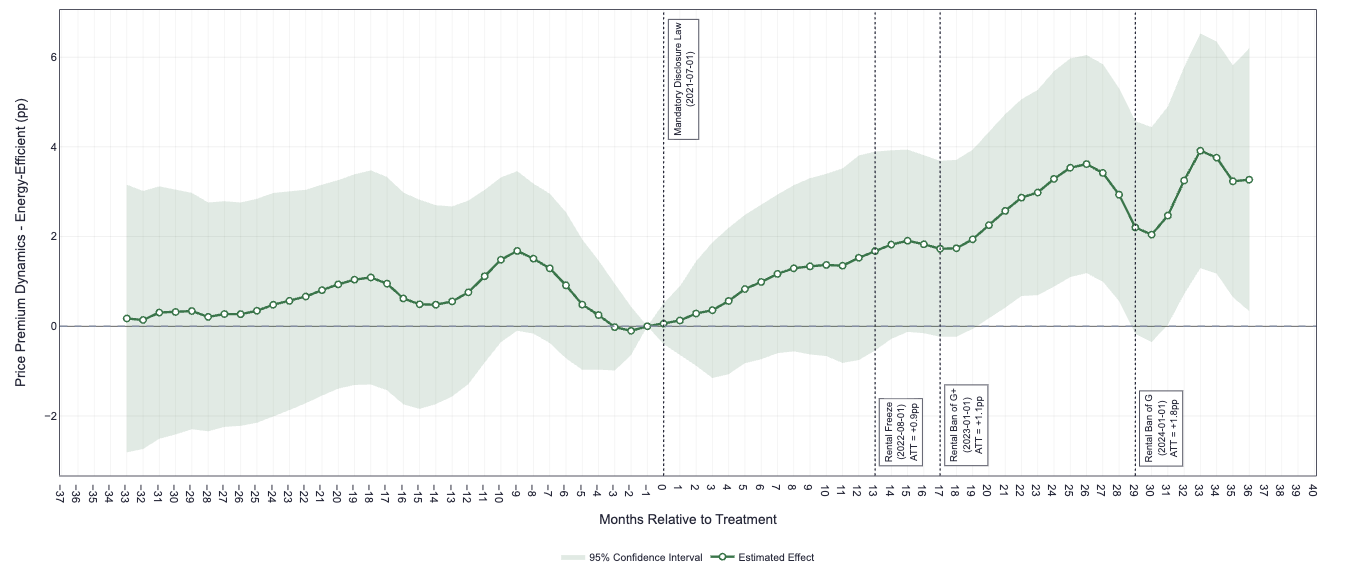
\includegraphics[width=\textwidth]{fig/event-study/apartment/index/event-study-efficient.png} 
        \label{fig:row1_1}
    \end{subfigure} 
    \begin{subfigure}{0.49\textwidth}
        \centering
        \caption{Houses Up for Sale (Full sample)}
        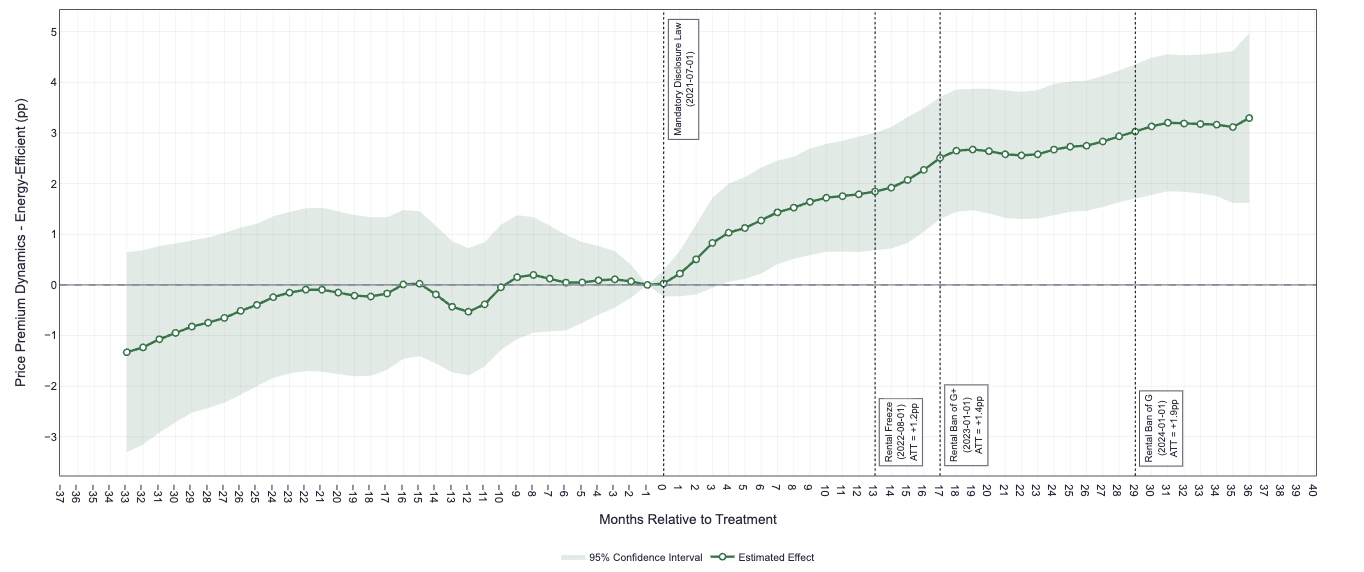
\includegraphics[width=\textwidth]{fig/event-study/house/index/event-study-efficient.png} 
        \label{fig:row1_2}
    \end{subfigure}

    \vspace{.5em} % Vertical space between rows

    % Intensive
    \begin{subfigure}{0.49\textwidth}
        \centering
        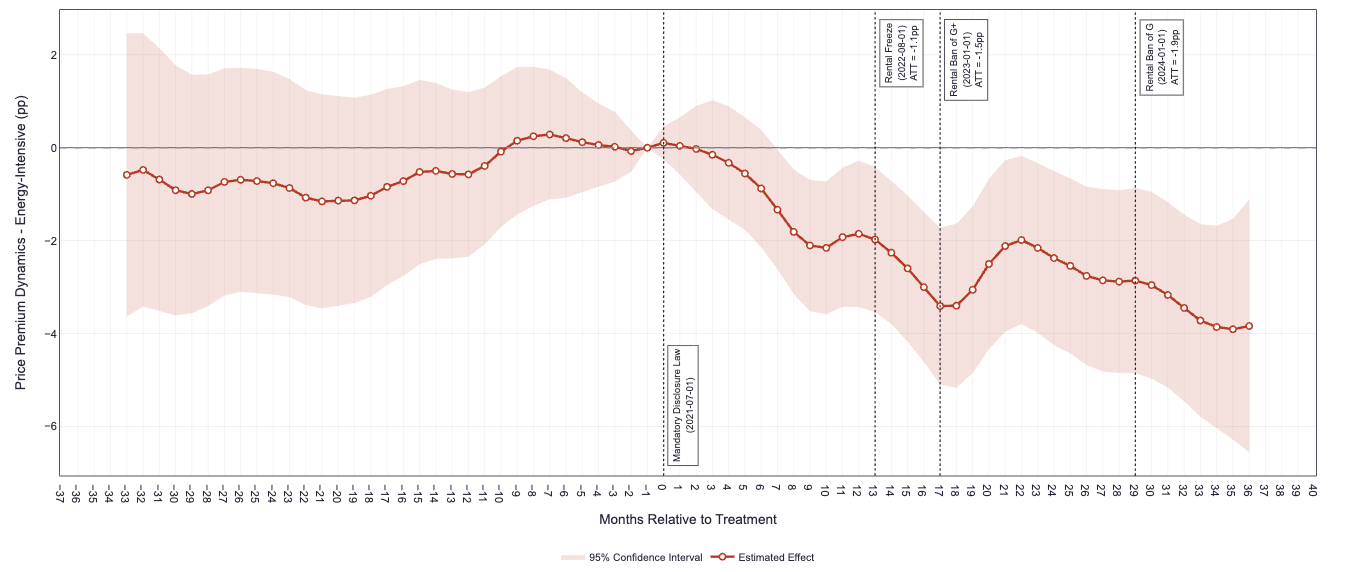
\includegraphics[width=\textwidth]{fig/event-study/apartment/index/event-study-intensive.png} 
    \end{subfigure} 
    \begin{subfigure}{0.49\textwidth}
        \centering
        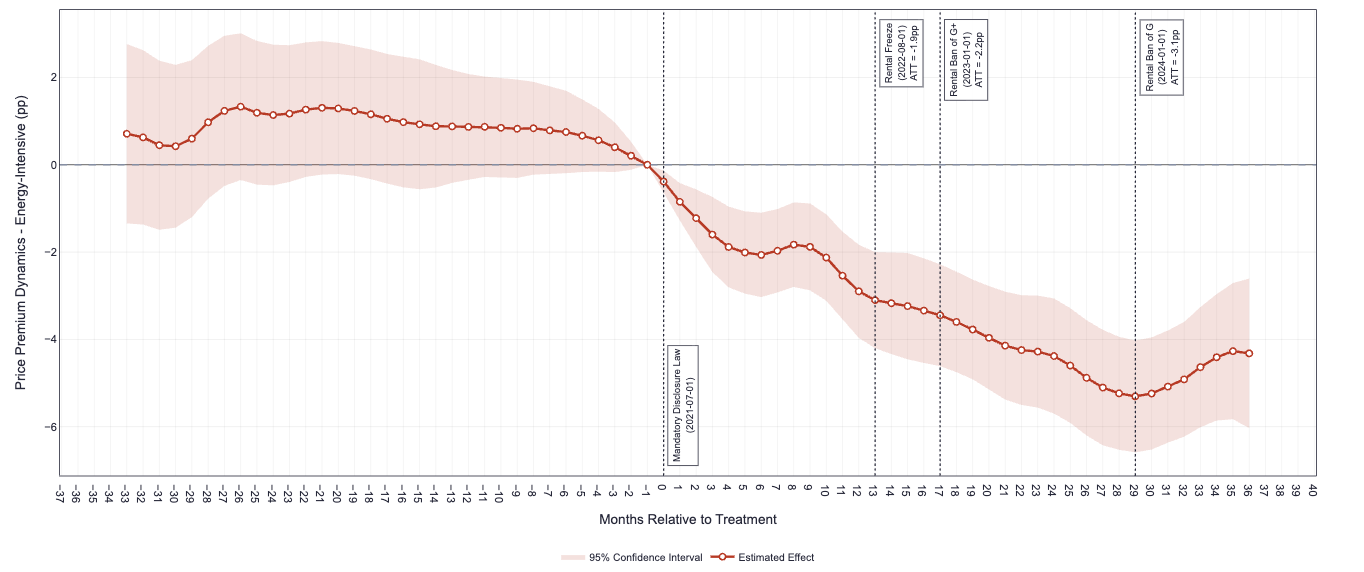
\includegraphics[width=\textwidth]{fig/event-study/house/index/event-study-intensive.png} 
        \label{fig:row2_2}
    \end{subfigure}

    \vspace{.5em} % Vertical space between rows

    % Missing
    \begin{subfigure}{0.49\textwidth}
        \centering
        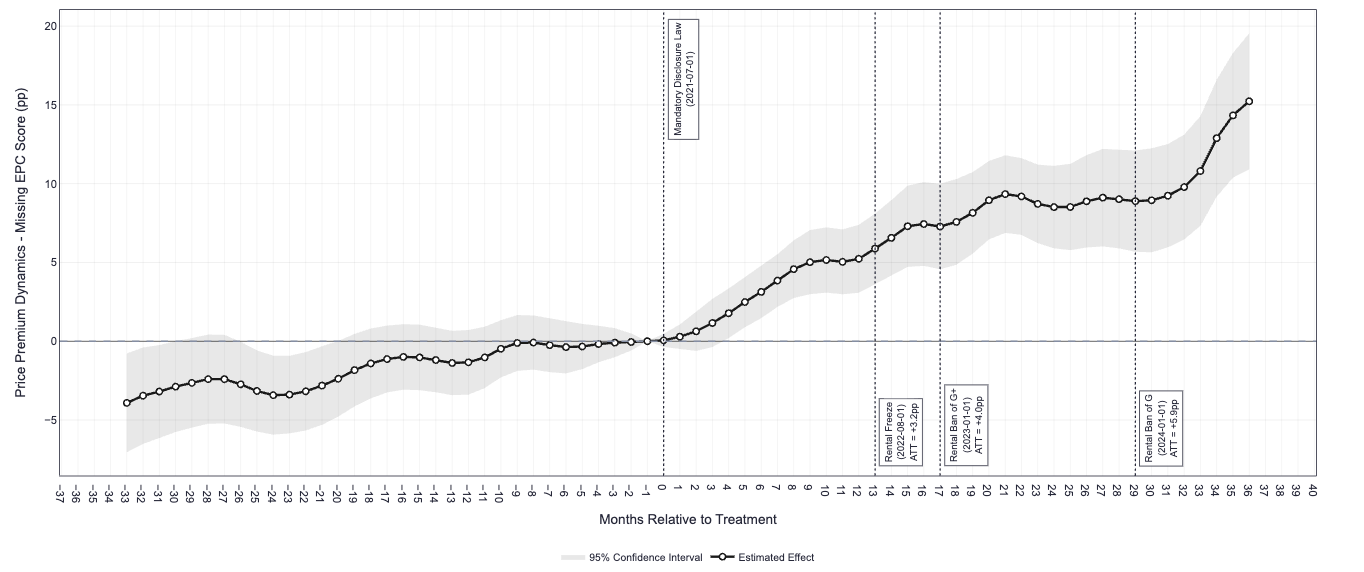
\includegraphics[width=\textwidth]{fig/event-study/apartment/index/event-study-missing.png} 
    \end{subfigure} 
    \begin{subfigure}{0.49\textwidth}
        \centering
        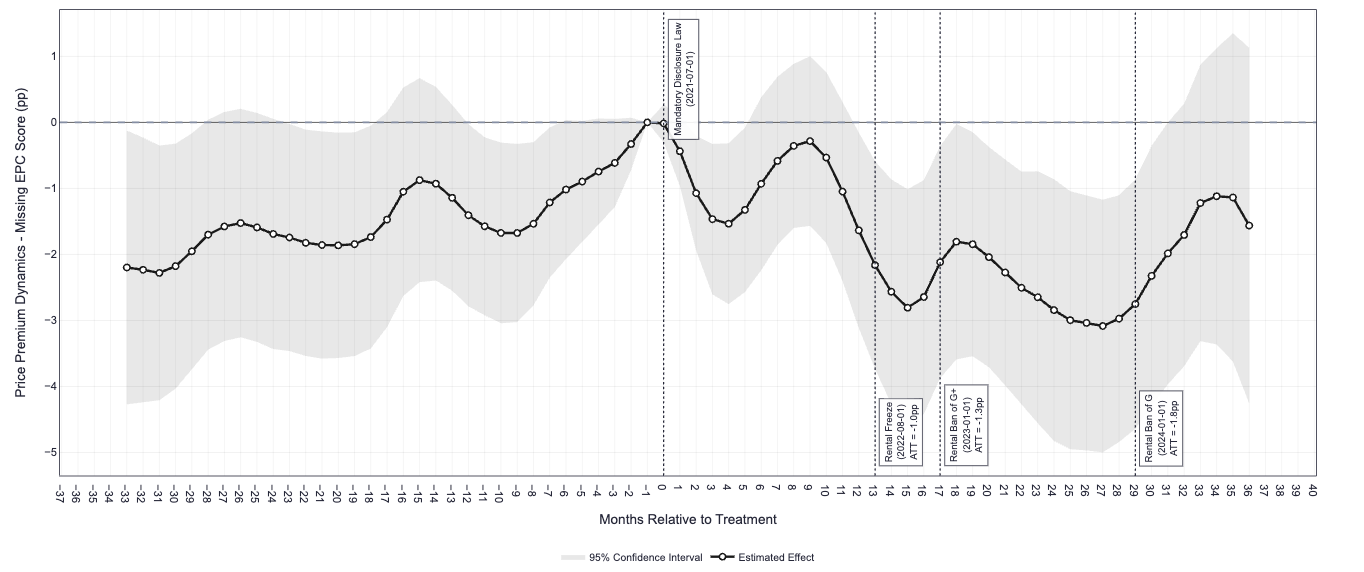
\includegraphics[width=\textwidth]{fig/event-study/house/index/event-study-missing.png} 
    \end{subfigure} 
    \label{fig:ATT}
    \begin{minipage}{\textwidth}
    \vspace{0.5em} 
        \footnotesize{\textbf{Note.} The panels present event-study estimates from the second step of our two-step hedonic procedure (see chapter one). Each series plots the monthly change in hedonic listing prices of the reference property around the introduction of mandatory EPC disclosure, separately by energy-consumption group and property type.  Shaded bands represent 95\% confidence intervals. These dynamics trace how the policy’s effect on predicted apartment and house prices evolves before and after the disclosure requirement in July 2021.}
    \end{minipage}
\end{figure}
\clearpage
\begin{figure}[H]
    \centering
    \caption{Visual representation of the model dynamics}
    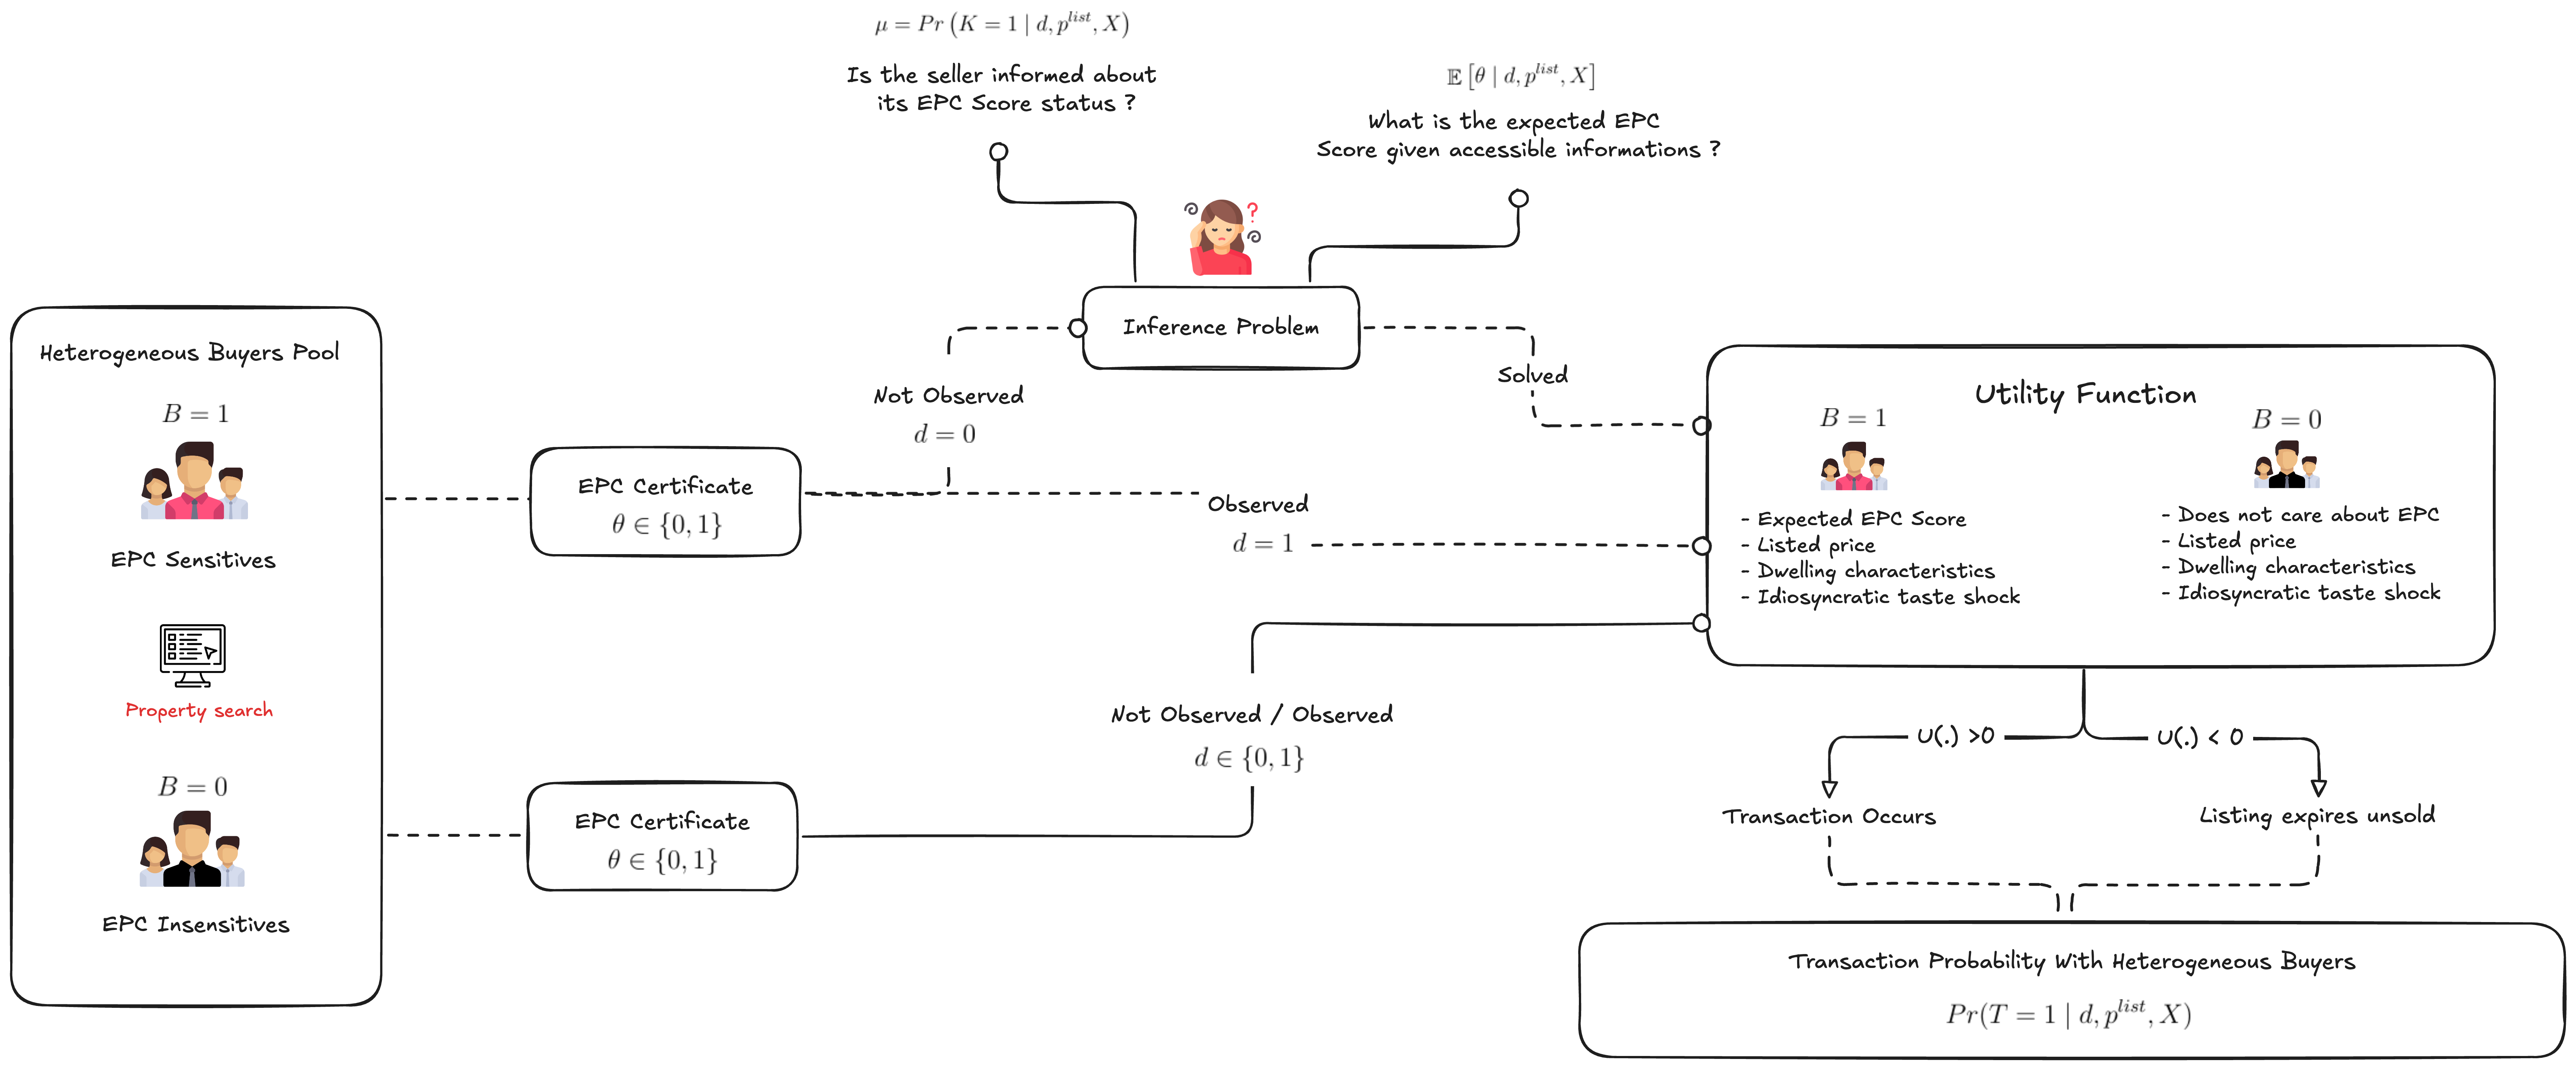
\includegraphics[width=1\textwidth]{fig/visuals/model_mechanics_overview_h.png} 
    \label{fig:vis_model}
\end{figure}

\section{Data and Model Objects}

Our dataset includes residential property listings from various French housing markets. For each listing $i$ in market $m$, we observe:

\begin{itemize}
\item $p_i$: listing price
\item $X_i$: vector of property characteristics (such as size, age, location, etc.)
\item $d_i \in {0,1}$: indicator of whether the Energy Performance Certificate (EPC) score is displayed in the listing
\item $\text{EPC}_i^{\text{listing}}$: the EPC score displayed on the listing (if $d_i = 1$)
\end{itemize}

What sets this approach apart is our ability to match these listings with data from ADEME (the French Environment and Energy Management Agency), which maintains an official registry of certified energy audits. These audits are reported by third-party assessors who are presumed to be honest and impartial. We match listings to the ADEME registry based on key characteristics that are registered in both databases, such as addresses, floor, item type, and area\footnote{We provide a full explanation of our matching strategy in the appendix}. This allows us to assess the accuracy of the EPC scores displayed in listings by comparing them to the official certified energy audits. This allows us to observe notably:

\begin{itemize}
    \item $K_i \in \{0,1\}$: whether a verified EPC exists at listing time
    \item $\theta_i$: the true (verified) EPC score (if $K_i = 1$)
\end{itemize}

This matching generates four mutually exclusive groups:

\begin{table}[H]
\centering
\caption{Classification of Listings}
\label{tab:listing_types}
\renewcommand{\arraystretch}{1.4}
\begin{tabular}{lccl}
\toprule
\toprule
\textbf{Group} & \textbf{Displays EPC} ($d_i$) & \textbf{Verified EPC Exists} ($K_i$) & \textbf{Interpretation} \\
\midrule
Truthful Disclosure & 1 & 1 & Informed seller reveals $\theta$ \\
Strategic Hiding & 0 & 1 & Informed seller conceals $\theta$ \\
Uninformed & 0 & 0 & Seller lacks information \\
Falsification & 1 & 0 or mismatch & Misreporting (excluded) \\
\bottomrule
\bottomrule
\end{tabular}
\end{table}

The key identification advantage is that we directly observe the latent variable $K_i$ (information status), which the model treats as unobservable to buyers. This allows us to separately identify the behavior of informed and uninformed sellers.


\section{Proofs}
\label{app:proofs}

All results below adopt the benchmark $\alpha_k=\beta_k$.

%------------------------------------------------------------
\subsection*{Preliminary: Optimal Price Sensitivity to Buyer Valuation}

\begin{proof}[Optimal price sensitivity to shifts in buyer valuation]

The optimal price $p^*$ satisfies the first-order condition:
\begin{equation}
    \frac{\gamma_1}{\gamma_0 + \gamma_1 \cdot p^*} = 1 - G(v_1 - p^*)
\end{equation}

Define the left-hand side as $\mathrm{LHS}(p) = \frac{\gamma_1}{\gamma_0 + \gamma_1 \cdot p}$ and the right-hand side as $\mathrm{RHS}(p; v_1) = 1 - G(v_1 - p)$. The optimal price is determined by the intersection $\mathrm{LHS}(p^*) = \mathrm{RHS}(p^*; v_1)$.

\textbf{Monotonicity of each side in $p$.}

The left-hand side is strictly decreasing in $p$:
\begin{equation}
    \frac{\partial \mathrm{LHS}}{\partial p} = -\frac{\gamma_1^2}{(\gamma_0 + \gamma_1 \cdot p)^2} < 0
\end{equation}

The right-hand side is strictly increasing in $p$. Since $G$ is the logistic CDF, $G'(x) = G(x)(1 - G(x)) > 0$ for all $x$. Therefore:
\begin{equation}
    \frac{\partial \mathrm{RHS}}{\partial p} = G'(v_1 - p) > 0
\end{equation}

A strictly decreasing function intersects a strictly increasing function at most once, so $p^*$ is unique.

\textbf{Effect of $v_1$ on the right-hand side.}

At any fixed $p$, the right-hand side is strictly decreasing in $v_1$:
\begin{equation}
    \frac{\partial \mathrm{RHS}}{\partial v_1} = -G'(v_1 - p) < 0
\end{equation}

An increase in $v_1$ shifts the RHS curve downward.

\textbf{Comparative static.}

Using the chain rule, differentiating the equilibrium condition with respect to $v_1$:
\begin{equation}
    \frac{\partial \mathrm{LHS}}{\partial p} \cdot \frac{\partial p^*}{\partial v_1} = \frac{\partial \mathrm{RHS}}{\partial p} \cdot \frac{\partial p^*}{\partial v_1} + \frac{\partial \mathrm{RHS}}{\partial v_1}
\end{equation}

Rearranging:
\begin{equation}
    \frac{\partial p^*}{\partial v_1} = \frac{\frac{\partial \mathrm{RHS}}{\partial v_1}}{\frac{\partial \mathrm{LHS}}{\partial p} - \frac{\partial \mathrm{RHS}}{\partial p}} = \frac{-G'(v_1 - p^*)}{-\frac{\gamma_1^2}{(\gamma_0 + \gamma_1 \cdot p^*)^2} - G'(v_1 - p^*)} > 0
\end{equation}

The numerator is negative. The denominator is negative (sum of two negative terms). Therefore $\frac{\partial p^*}{\partial v_1} > 0$.
\end{proof}

%------------------------------------------------------------
\subsection*{Lemma A.1 (Profit is Increasing in Sensitive-Buyer Valuation)}
\label{lem:profit}

\textit{Holding $v_0$ and $\rho$ fixed, the gross profit function $\tilde{\Pi}(v_1; v_0, \rho)$ is strictly increasing in $v_1$ whenever $\rho > 0$.}

\begin{proof}[Proof of Lemma A.1]
Let $p_{\mathrm{list}}^*(v_1)$ denote the optimal price given sensitive-buyer valuation $v_1$. By the envelope theorem, the effect of a small increase in $v_1$ on maximized profit is:
\begin{equation}
    \frac{\partial \tilde{\Pi}}{\partial v_1} = \phi(p_{\mathrm{list}}^*) \cdot \rho \cdot G'(v_1 - p_{\mathrm{list}}^*)
\end{equation}
where we evaluate the partial derivative of the objective holding $p$ fixed at the optimum.

All three terms are positive: $\phi(p^*) > 0$ (expected transaction price is positive), $\rho \in [0,1] \geq 0$ (by assumption), and $G'(\cdot) > 0$ (logistic density is everywhere positive). Therefore $\frac{\partial \tilde{\Pi}}{\partial v_1} > 0$.
\end{proof}

Since $\tilde{\Pi}$ is increasing in $v_1$, the profit gain from disclosure is positive if and only if $v_1(d=1) > v_1(d=0)$: sensitive buyers value the property more when quality is revealed than when it is hidden. In this case, disclosure raises profit, and the seller discloses (absent hiding costs). Conversely, the profit gain is negative if $v_1(d=1) < v_1(d=0)$: sensitive buyers value the property more under hiding. This occurs when buyers' inference about non-disclosers is more favorable than the truth. In this case, hiding raises profit, and the seller hides (absent sufficiently high hiding costs).

%------------------------------------------------------------
\subsection*{Proof of Proposition \ref{prop:premium} (Non-Disclosure Premium)}

\begin{proof}
By Lemma A.1, $p^*_0 > p^*_1$ if and only if $v_1(d=0) > v_1(d=1, \theta)$. Since $v_1(d=0) - v_1(d=1, \theta) = \beta_1 \cdot (\mathbb{E}[\theta \mid d=0] - \theta)$ and $\beta_1 > 0$, this holds if and only if $\mathbb{E}[\theta \mid d=0] > \theta$.

\begin{itemize}
    \item \textbf{For a low-quality seller} ($\theta = 0$): the condition is $\mathbb{E}[\theta \mid d=0] > 0$, which holds whenever the non-disclosing pool contains any high-quality sellers.
    \item \textbf{For a high-quality seller} ($\theta = 1$): the condition is $\mathbb{E}[\theta \mid d=0] > 1$, which is impossible since $\theta \in \{0,1\}$.
\end{itemize}
\end{proof}

%------------------------------------------------------------
\subsection*{Proof of Corollary \ref{cor:hq_disclose} (High-Quality Sellers Always Disclose)}

\begin{proof}
From Proposition \ref{prop:premium}, the non-disclosure premium exists if and only if $\mathbb{E}[\theta \mid d=0] > \theta$.

For a high-quality seller ($\theta = 1$), this condition requires $\mathbb{E}[\theta \mid d=0] > 1$. But $\theta \in \{0, 1\}$, so $\mathbb{E}[\theta \mid d=0] \leq 1$ always. Therefore the condition never holds: high-quality sellers never earn a premium from hiding.

In fact, the inequality is strict whenever the non-disclosing pool contains any low-quality sellers. In that case $\mathbb{E}[\theta \mid d=0] < 1$, so:
\begin{equation}
    v_1(d=1, \theta=1) - v_1(d=0) = \beta_1 \cdot (1 - \mathbb{E}[\theta \mid d=0]) > 0
\end{equation}

Disclosure yields a strictly higher valuation, and therefore strictly higher profit. Adding hiding costs $C(\theta=1) = c_0 + c_1 \geq 0$ only reinforces this: disclosure dominates hiding.
\end{proof}

%------------------------------------------------------------
\subsection*{Proof of Proposition \ref{prop:pi} (Non-disclosure premium is decreasing in $\pi$)}

\begin{proof}
From Eq.~\eqref{eq:mu}, the posterior $\mu = \Pr(K=1 \mid d=0)$ is increasing in $\pi$: when $\pi \to 0$, $\mu \to 0$; when $\pi \to 1$, $\mu \to 1$.

From Eq.~\eqref{eq:belief}:
\begin{equation}
    \mathbb{E}[\theta \mid d=0] = \mu \cdot \Pr(\theta=1 \mid K=1, d=0) + (1-\mu) \cdot \Pr(\theta=1 \mid K=0)
\end{equation}

Taking the derivative with respect to $\mu$:
\begin{equation}
    \frac{\partial \mathbb{E}[\theta \mid d=0]}{\partial \mu} = \Pr(\theta=1 \mid K=1, d=0) - \Pr(\theta=1 \mid K=0)
\end{equation}

We assume that information status is independent of quality: $K \perp \theta$. This means whether a seller obtains an audit is unrelated to the property's actual energy efficiency. For instance, audits are delayed due to administrative reasons, not avoided due to anticipated bad news. Under this assumption:
\begin{equation}
    \Pr(\theta=1 \mid K=0) = \Pr(\theta=1) = \bar{\theta}
\end{equation}

By Bayes' rule:
\begin{equation}
    \Pr(\theta=1 \mid K=1, d=0) = \frac{\Pr(d=0 \mid K=1, \theta=1) \cdot \Pr(\theta=1 \mid K=1)}{\Pr(d=0 \mid K=1)}
\end{equation}

By the independence assumption, $\Pr(\theta=1 \mid K=1) = \bar{\theta}$. Expanding the denominator by the law of total probability:
\begin{equation}
    \Pr(\theta=1 \mid K=1, d=0) = \frac{\Pr(d=0 \mid K=1, \theta=1) \cdot \bar{\theta}}{\Pr(d=0 \mid K=1, \theta=1) \cdot \bar{\theta} + \Pr(d=0 \mid K=1, \theta=0) \cdot (1-\bar{\theta})}
\end{equation}

This expression is less than $\bar{\theta}$ if and only if:
\begin{equation}
    \begin{split}
        &\Pr(d=0 \mid K=1, \theta=1) \cdot \bar{\theta} < \bar{\theta} \cdot \left[ \Pr(d=0 \mid K=1, \theta=1) \cdot \bar{\theta} + \Pr(d=0 \mid K=1, \theta=0) \cdot (1-\bar{\theta}) \right] \\[0.5em]
    \Longleftrightarrow\;& \Pr(d=0 \mid K=1, \theta=1) < \Pr(d=0 \mid K=1, \theta=1) \cdot \bar{\theta} + \Pr(d=0 \mid K=1, \theta=0) \cdot (1-\bar{\theta}) \\[0.5em]
    \Longleftrightarrow\;& \Pr(d=0 \mid K=1, \theta=1) \cdot (1-\bar{\theta}) < \Pr(d=0 \mid K=1, \theta=0) \cdot (1-\bar{\theta}) \\[0.5em]
    \Longleftrightarrow\;& \Pr(d=0 \mid K=1, \theta=1) < \Pr(d=0 \mid K=1, \theta=0)
    \end{split}
\end{equation}

That is, high-quality informed sellers hide less often than low-quality informed sellers. This follows from Corollary \ref{cor:hq_disclose}: high-quality sellers gain from disclosure ($v_1(d=1) > v_1(d=0)$ when $\theta=1$), while low-quality sellers gain from hiding ($v_1(d=0) > v_1(d=1)$ when $\theta=0$).

Therefore:
\begin{equation}
    \frac{\partial \mathbb{E}[\theta \mid d=0]}{\partial \mu} = \underbrace{\Pr(\theta=1 \mid K=1, d=0)}_{< \bar{\theta}} - \underbrace{\Pr(\theta=1 \mid K=0)}_{= \bar{\theta}} < 0
\end{equation}

By the chain rule:
\begin{equation}
    \frac{\partial \mathbb{E}[\theta \mid d=0]}{\partial \pi} = \underbrace{\frac{\partial \mathbb{E}[\theta \mid d=0]}{\partial \mu}}_{<0} \cdot \underbrace{\frac{\partial \mu}{\partial \pi}}_{>0} < 0
\end{equation}

From Proposition \ref{prop:premium}, the premium is increasing in $\mathbb{E}[\theta \mid d=0] - \theta$. Since $\mathbb{E}[\theta \mid d=0]$ is decreasing in $\pi$, the premium is decreasing in $\pi$. When $\pi$ is low, most non-disclosers are uninformed. They hide because they lack information, not because they have bad news to conceal. Buyers recognize this and treat non-disclosure leniently, expecting quality close to the population average $\bar{\theta}$. A low-quality seller benefits from this forgiving environment: she is pooled with uninformed sellers who may have good properties. When $\pi$ is high, most non-disclosers are informed sellers who chose to hide. Since high-quality informed sellers prefer to disclose, the hiding pool is dominated by low-quality types. Buyers recognize this and penalize non-disclosure harshly, expecting quality close to zero. The low-quality seller can no longer hide among uninformed sellers (there are too few of them) and the premium vanishes.
\end{proof}

%------------------------------------------------------------
\subsection*{Proof of Proposition \ref{prop:rho} (Non-disclosure premium is increasing in $\rho$)}

\begin{proof}
Recall from Eq.~\eqref{eq:demand} that the transaction probability writes:
\begin{equation}
    \Gamma(p \mid d) = \rho \cdot G(v_1(d) - p) + (1-\rho) \cdot G(v_0 - p)
\end{equation}

The seller maximizes $\Pi(p) = \phi(p) \cdot \Gamma(p \mid d)$ where $\phi(p) = \gamma_0 + \gamma_1 \cdot p$.

\begin{itemize}
    \item \textbf{Case $\rho = 0$.} The economy is only composed of EPC-insensitive buyers. The transaction probability reduces to:
    \begin{equation}
        \Gamma(p \mid d) = G(v_0 - p)
    \end{equation}
    This is independent of $d$: the demand curve is the same under disclosure and hiding. Therefore the optimal price is the same: $p^*_0 = p^*_1$, and the premium is zero.

    \item \textbf{Case $\rho = 1$.} The economy is only composed of EPC-sensitive buyers. The transaction probability reduces to:
    \begin{equation}
        \Gamma(p \mid d) = G(v_1(d) - p)
    \end{equation}
    The demand curve under hiding is $G(v_1(d=0) - p)$. The demand curve under disclosure is $G(v_1(d=1) - p)$. For a low-quality seller with $\mathbb{E}[\theta \mid d=0] > 0$:
    \begin{equation}
        v_1(d=0) > v_1(d=1, \theta=0)
    \end{equation}
    The demand curve under hiding is shifted to the right relative to disclosure. A rightward shift in demand leads to a higher optimal price: $p^*_0 > p^*_1$. The premium is maximized.

    \item \textbf{Monotonicity in $\rho$.} Consider the demand curves under hiding and disclosure:
    \begin{align}
        \Gamma(p \mid d=0) &= \rho \cdot G(v_1(d=0) - p) + (1-\rho) \cdot G(v_0 - p) \\
        \Gamma(p \mid d=1) &= \rho \cdot G(v_1(d=1) - p) + (1-\rho) \cdot G(v_0 - p)
    \end{align}

    The difference between these demand curves is:
    \begin{equation}
        \Gamma(p \mid d=0) - \Gamma(p \mid d=1) = \rho \cdot \left[ G(v_1(d=0) - p) - G(v_1(d=1) - p) \right]
    \end{equation}

    For a low-quality seller with $v_1(d=0) > v_1(d=1, \theta=0)$, and since $G$ is increasing, the term in brackets is positive. Therefore the difference in demand curves is proportional to $\rho$: when $\rho = 0$, the demand curves are identical; as $\rho$ increases, they diverge.

    At $\rho = 0$, the seller faces the same demand curve under both regimes, so $p^*_0 = p^*_1$.

    As $\rho$ increases, the demand curve under hiding shifts rightward relative to disclosure (because more weight is placed on the higher valuation $v_1(d=0)$). A rightward shift in demand increases the optimal price. Therefore $p^*_0$ increases relative to $p^*_1$, and the premium $p^*_0 - p^*_1$ increases.
\end{itemize}

The premium exists because sensitive buyers value non-disclosing properties more than disclosing ones (for low-quality sellers). When $\rho = 0$, there are no sensitive buyers, so this valuation difference is irrelevant (both regimes face the same demand). As $\rho$ increases, sensitive buyers constitute a larger share of the market, and their favorable view of non-disclosure translates into higher demand and higher prices for hiding sellers. The premium grows because the ``audience'' that is sensitive to energy performance is getting larger.
\end{proof}

%------------------------------------------------------------
\subsection*{Proof of Proposition \ref{prop:equilibrium} (Equilibrium Existence and Uniqueness)}

\begin{proof}
There exists a unique equilibrium.

\vspace{.5em}

\textbf{Full Unraveling.} Suppose $c_0 > \Delta(\bar{\theta})$, i.e., $\Phi(0) < 0$.

Consider the most favorable scenario for hiding: $\sigma_0 = 0$, so only uninformed sellers hide and pool quality equals $\bar{\theta}$. Even in this best case, hiding is unprofitable: $\Delta(\bar{\theta}) < c_0$.

Since $\Phi$ is decreasing, $\Phi(\sigma_0) < \Phi(0) < 0$ for all $\sigma_0 > 0$. Hiding is never profitable. The unique equilibrium has $\sigma_0^* = 0$.

\textit{Full Unraveling} occurs when hiding costs are high relative to the benefit. Even under the most favorable beliefs (pool quality $\bar{\theta}$), the profit gain from hiding does not justify the cost. All informed sellers disclose. The non-disclosing pool contains only uninformed sellers, and buyers correctly infer average quality. This is the classical \cite{grossman_informational_1981}--\cite{milgrom_good_1981} outcome but achieved through high hiding costs rather than through complete information.

\vspace{.5em}

\textbf{Partial Separation.} Suppose $c_0 < \Delta(e(1))$, i.e., $\Phi(1) > 0$.

Consider the least favorable scenario for hiding: $\sigma_0 = 1$, so all low-quality sellers hide and pool quality falls to $e(1)$. Even in this worst case, hiding is profitable: $\Delta(e(1)) > c_0$.

Since $\Phi$ is decreasing and $\Phi(1) > 0$, we have $\Phi(\sigma_0) > 0$ for all $\sigma_0 \in [0,1]$. Hiding is always profitable. The unique equilibrium has $\sigma_0^* = 1$.

\textit{Partial Separation} occurs when hiding costs are low. Even under the least favorable beliefs (pool quality $e(1)$), hiding remains profitable for low-quality sellers. High-quality informed sellers disclose to separate; low-quality informed sellers hide to pool with uninformed sellers. Buyers understand this and discount non-disclosers accordingly, but the discount is limited by the presence of uninformed sellers, who provide cover.

\vspace{.5em}

\textbf{Mixed Strategy.} Suppose $\Delta(e(1)) \leq c_0 \leq \Delta(\bar{\theta})$, i.e., $\Phi(1) \leq 0 \leq \Phi(0)$.

At $\sigma_0 = 0$: hiding would be profitable ($\Phi(0) \geq 0$), so some sellers want to deviate to hiding.

At $\sigma_0 = 1$: hiding would be unprofitable ($\Phi(1) \leq 0$), so some sellers want to deviate to disclosure.

By continuity and strict monotonicity of $\Phi$, there exists a unique $\sigma_0^* \in (0,1)$ such that $\Phi(\sigma_0^*) = 0$. At this point, low-quality sellers are exactly indifferent between hiding and disclosing, sustaining a mixed strategy.

\textit{Mixed Strategy} is the knife-edge case. The hiding cost exactly equals the profit gain at some interior belief. Low-quality sellers randomize to keep buyers' beliefs at the indifference point. This case is non-generic and unlikely to be empirically relevant.

\textbf{Uniqueness:} In all three cases, uniqueness follows from strict monotonicity of $\Phi$. There is exactly one value of $\sigma_0$ consistent with equilibrium.
\end{proof}

%------------------------------------------------------------
\subsection*{Proof of Proposition \ref{prop:pi} (Equilibrium effect of $\pi$: equilibrium moves toward full unraveling)}

\begin{proof}
From Eq.~\eqref{eq:belief_simplified}, the equilibrium belief under partial separation is:
\begin{equation}
    e(1) = \frac{(1-\pi)\bar{\theta}}{1 - \pi\bar{\theta}}
\end{equation}

Taking the derivative:
\begin{equation}
    \frac{\partial e(1)}{\partial \pi} = \frac{-\bar{\theta}(1-\pi\bar{\theta}) - (1-\pi)\bar{\theta}(-\bar{\theta})}{(1-\pi\bar{\theta})^2} = \frac{-\bar{\theta}(1-\bar{\theta})}{(1-\pi\bar{\theta})^2} < 0
\end{equation}

As $\pi$ increases, $e(1)$ falls: the pool quality under partial separation deteriorates because fewer uninformed sellers are available to provide cover.

Since $\Delta(e)$ is increasing in $e$, $\Delta(e(1))$ falls. The condition for partial separation, $c_0 < \Delta(e(1))$, becomes harder to satisfy. For fixed $c_0$, an increase in $\pi$ can push the equilibrium from partial separation into the mixed or full unraveling region.
\end{proof}

When most sellers are informed ($\pi$ high), non-disclosure is suspicious. Buyers recognize that uninformed sellers are rare, so most non-disclosers must be strategic hiders. The favorable cover provided by uninformed sellers evaporates. Low-quality sellers find hiding less attractive, and the market approaches classical unraveling.

%------------------------------------------------------------
\subsection*{Proof of Proposition \ref{prop:rho} (Equilibrium effect of $\rho$: equilibrium moves toward partial separation)}

\begin{proof}
The profit gain from hiding is:
\begin{equation}
    \Delta(e) = \Pi(d=0) - \Pi(d=1, \theta=0)
\end{equation}

From Proposition \ref{prop:rho}, this gap is increasing in $\rho$. When more buyers are sensitive to quality, the valuation difference $v_1(d=0) - v_1(d=1, \theta=0) = \beta_1 \cdot e$ translates more strongly into revenue differences.

As $\rho$ increases, both $\Delta(\bar{\theta})$ and $\Delta(e(1))$ increase. The condition for partial separation, $c_0 < \Delta(e(1))$, becomes easier to satisfy. For fixed $c_0$, an increase in $\rho$ can push the equilibrium from full unraveling into the mixed or partial separation region.
\end{proof}

When most buyers care about quality ($\rho$ high), the stakes of disclosure are high. Low-quality sellers have much to lose from revealing their type. The non-disclosure premium is large, making hiding attractive even when pool quality is low. Partial separation is sustained.

%------------------------------------------------------------
\subsection*{Proof of Proposition \ref{prop:c0} (Equilibrium effect of $c_0$: equilibrium moves toward full unraveling)}

\begin{proof}
An increase in $c_0$ shifts the function $\Phi(\sigma_0) = \Delta(e(\sigma_0)) - c_0$ downward. The boundaries become:
\begin{equation}
    \begin{split}
        \Phi(0) &= \Delta(\bar{\theta}) - c_0 \quad \text{(decreases)} \\
        \Phi(1) &= \Delta(e(1)) - c_0 \quad \text{(decreases)}
    \end{split}
\end{equation}

The condition for full unraveling, $c_0 > \Delta(\bar{\theta})$, becomes easier to satisfy. The condition for partial separation, $c_0 < \Delta(e(1))$, becomes harder to satisfy.
\end{proof}

Higher hiding costs make concealment less attractive. Regulatory enforcement, administrative burden, or reputational concerns that raise $c_0$ push the market toward disclosure.

%------------------------------------------------------------
\subsection*{Proof of Proposition \ref{prop:subsidy} (Subsidy Comparative Statics)}

\subsubsection*{Effect of $\pi$ on the renovation threshold ($\partial\bar{R}/\partial\pi > 0$)}

\begin{proof}
Recall from Eq.~\eqref{eq:threshold} that $\bar{R} = \Pi(d=1, \theta=1) - \Pi(d=0) + c_0$.

The revenue from disclosing high quality, $\Pi(d=1, \theta=1)$, does not depend on $\pi$. Under disclosure, buyers observe $\theta = 1$ directly; their valuation is independent of the composition of non-disclosers (see Corollary \ref{cor:hq_disclose}).

The revenue from hiding, $\Pi(d=0)$, depends on $\pi$ through buyers' inference. From Proposition \ref{prop:pi}, $\mathbb{E}[\theta \mid d=0]$ is decreasing in $\pi$: when more sellers are informed, buyers attribute non-disclosure to strategic hiding and infer lower quality. Lower inferred quality reduces the sensitive buyers' valuation $v_1(d=0)$, which reduces demand and therefore revenue. Hence $\Pi(d=0)$ is decreasing in $\pi$.

Since $\Pi(d=1, \theta=1)$ is constant in $\pi$ and $\Pi(d=0)$ is decreasing in $\pi$:
\begin{equation}
    \frac{\partial \bar{R}}{\partial \pi} = -\frac{\partial \Pi(d=0)}{\partial \pi} > 0
\end{equation}
\end{proof}

When few sellers are informed ($\pi$ low), hiding is attractive: buyers forgive non-disclosure, and the revenue $\Pi(d=0)$ is high. The gain from renovating (switching from hiding to disclosing high quality) is therefore small. Only cheap renovations are worthwhile.

When most sellers are informed ($\pi$ high), hiding is penalized: buyers suspect strategic concealment, and $\Pi(d=0)$ is low. The gain from renovating is large, it offers a substantial upgrade over the poor hiding payoff. Expensive renovations become worthwhile.

\subsubsection*{Effect of $\rho$ on the renovation threshold ($\partial\bar{R}/\partial\rho > 0$)}

\begin{proof}
Recall from Eq.~\eqref{eq:threshold} that $\bar{R} = \Pi(d=1, \theta=1) - \Pi(d=0) + c_0$. Since $c_0$ does not depend on $\rho$:
\begin{equation}
    \frac{\partial \bar{R}}{\partial \rho} = \frac{\partial}{\partial \rho}\left[ \Pi(d=1, \theta=1) - \Pi(d=0) \right]
\end{equation}

Consider the demand curves under disclosing $\theta=1$ and under hiding:
\begin{align}
    \Gamma(p \mid d=1, \theta=1) &= \rho \cdot G(v_1(d=1, \theta=1) - p) + (1-\rho) \cdot G(v_0 - p) \\
    \Gamma(p \mid d=0) &= \rho \cdot G(v_1(d=0) - p) + (1-\rho) \cdot G(v_0 - p)
\end{align}

The difference is:
\begin{equation}
    \Gamma(p \mid d=1, \theta=1) - \Gamma(p \mid d=0) = \rho \cdot \left[ G(v_1(d=1, \theta=1) - p) - G(v_1(d=0) - p) \right]
\end{equation}

Since $v_1(d=1, \theta=1) = \beta_0 + \beta_1 + \sum_n \beta_n X_n$ and $v_1(d=0) = \beta_0 + \beta_1 \mathbb{E}[\theta \mid d=0] + \sum_n \beta_n X_n$:
\begin{equation}
    v_1(d=1, \theta=1) - v_1(d=0) = \beta_1 (1 - \mathbb{E}[\theta \mid d=0]) > 0
\end{equation}

The inequality holds because $\mathbb{E}[\theta \mid d=0] < 1$ (the non-disclosing pool contains some low-quality sellers).

Since $v_1(d=1, \theta=1) > v_1(d=0)$ and $G$ is increasing, the term in brackets is positive. The demand gap is proportional to $\rho$: when $\rho = 0$, the demand curves are identical; as $\rho$ increases, they diverge, with the demand curve under disclosing $\theta=1$ shifting rightward relative to hiding. At $\rho = 0$, the seller faces the same demand curve under both regimes, so revenues are equal and $\Pi(d=1, \theta=1) - \Pi(d=0) = 0$. As $\rho$ increases, the demand curve under disclosing $\theta=1$ shifts rightward relative to hiding. A rightward shift in demand increases the optimal price and revenue. Therefore $\Pi(d=1, \theta=1)$ increases relative to $\Pi(d=0)$, and the gap $\Pi(d=1, \theta=1) - \Pi(d=0)$ increases.
\end{proof}

When no buyers are sensitive ($\rho = 0$), disclosure status is irrelevant for demand. The revenue from disclosing $\theta=1$ equals the revenue from hiding, so the gain from renovating is just the avoided hiding cost $c_0$.

When buyers are sensitive ($\rho > 0$), they value verified high quality more than the uncertain pool. Disclosing $\theta=1$ generates higher demand than hiding. As $\rho$ increases, more buyers respond to this quality difference, amplifying the revenue gain from renovation.

\textbf{Note:} This result may seem to contradict Proposition \ref{prop:rho}, which showed that the non-disclosure premium for low-quality sellers increases with $\rho$. There is no contradiction. The earlier result compared hiding versus disclosing $\theta=0$, where $v_1(d=0) > v_1(d=1, \theta=0)$ (hiding has the higher valuation). Here we compare disclosing $\theta=1$ versus hiding, where $v_1(d=1, \theta=1) > v_1(d=0)$ (disclosing has the higher valuation). In both cases, as $\rho$ increases, the regime with the higher valuation benefits more.

\subsubsection*{Effect of $c_0$ on the renovation threshold ($\partial\bar{R}/\partial c_0 = 1$)}

\begin{proof}
From the definition $\bar{R} = \Pi(d=1, \theta=1) - \Pi(d=0) + c_0$, and noting that $\Pi(d=1, \theta=1)$ and $\Pi(d=0)$ do not depend on $c_0$ (hiding costs are subtracted separately from revenue):
\begin{equation}
    \frac{\partial \bar{R}}{\partial c_0} = 1
\end{equation}
\end{proof}

A higher hiding cost makes hiding less attractive, euro for euro. Each additional euro of hiding cost raises the threshold by exactly one euro, making renovation relatively more attractive. This result implies that disclosure enforcement (which raises $c_0$) and renovation subsidies (which raise $S$) are perfect substitutes: both shift the renovation decision by the same amount per euro spent.

\subsubsection*{Optimal subsidy comparative statics ($\partial S^*/\partial\pi$, $\partial S^*/\partial\rho$, $\partial S^*/\partial\hat{R}$, $\partial S^*/\partial c_0$)}

\begin{proof}[Effect of $\pi$ on optimal subsidy]
From the definition $S^* = \max\{\hat{R}(X) - \bar{R}, 0\}$:
\begin{equation}
    \frac{\partial S^*}{\partial \pi} = -\frac{\partial \bar{R}}{\partial \pi} \leq 0
\end{equation}
where the inequality follows from the result above establishing $\frac{\partial \bar{R}}{\partial \pi} > 0$.
\end{proof}

Markets with more informed sellers have higher renovation thresholds: hiding is less attractive because buyers penalize non-disclosure. Private incentives to renovate are already strong, so smaller subsidies are needed.

\begin{proof}[Effect of $\rho$ on optimal subsidy]
From the definition $S^* = \max\{\hat{R}(X) - \bar{R}, 0\}$:
\begin{equation}
    \frac{\partial S^*}{\partial \rho} = -\frac{\partial \bar{R}}{\partial \rho} \leq 0
\end{equation}
where the inequality follows from the result above establishing $\frac{\partial \bar{R}}{\partial \rho} > 0$.
\end{proof}

Markets with more sensitive buyers have higher renovation thresholds: disclosing high quality commands a large premium. Private incentives to renovate are already strong, so smaller subsidies are needed.

\begin{proof}[Effect of $\hat{R}(X)$ on optimal subsidy]
When $\hat{R}(X) > \bar{R}$, we have $S^* = \hat{R}(X) - \bar{R}$, so:
\begin{equation}
    \frac{\partial S^*}{\partial \hat{R}(X)} = 1
\end{equation}
\end{proof}

Properties with higher renovation costs require proportionally higher subsidies. Each additional euro of renovation cost requires an additional euro of subsidy to maintain indifference.

\begin{proof}[Effect of $c_0$ on optimal subsidy]
From the definition $S^* = \hat{R}(X) - \bar{R}$ and $\bar{R} = \Pi(d=1, \theta=1) - \Pi(d=0) + c_0$:
\begin{equation}
    \frac{\partial S^*}{\partial c_0} = -\frac{\partial \bar{R}}{\partial c_0} = -1
\end{equation}
\end{proof}

Disclosure enforcement and renovation subsidies are perfect substitutes. Each euro spent on raising hiding costs (through fines, audits, or regulatory burden) reduces the required subsidy by exactly one euro. Policymakers can achieve the same renovation rate through either instrument.

% ============================================================
% BIBLIOGRAPHY
% ============================================================
\clearpage
\bibliographystyle{plainnat}
\bibliography{DPE_library}


\end{document}
